\documentclass{article}

% ****************************************************************
\usepackage{lipsum}		% Used to generate dummy-text (\lipsum[1])
\usepackage[margin=2.54cm,includefoot]{geometry}		% Used to control margins

\usepackage{graphicx} % allows to import images
\usepackage{float}	% allows for control of float positions
\usepackage{tikz} 	% Used to create trees



% Used for Header and Footer stuff
\usepackage{fancyhdr}
\pagestyle{fancy}
\fancyhead{}	% clears header
\fancyfoot{}	% clears footer
\fancyfoot[R]{\thepage}	% sets position right
\renewcommand{\headrulewidth}{0pt}	% removes header line by setting it to zero
\renewcommand{\footrulewidth}{1pt}		% add footer line by setting it to one
% ****************************************************************

\begin{document}

% ****************************************************************
\begin{titlepage}
	
	\begin{center}
	\line(1,0){330} \\
	[2mm]
	\huge{\bfseries Data Science Zusammenfassung} \\
	[2mm]
	\line(1,0){320} \\
	[1,5cm]
	\textsc{\LARGE By Yannis Schmutz} \\
	[0.75cm]
	\textsc{\large todo} \\
	
	\end{center}
	
\end{titlepage}
% ****************************************************************
\pagenumbering{roman}		% sets the page numbering to roman for the preface etc.
\section*{Zusammenfassung}	% Adds a section without a number in front
\addcontentsline{toc}{section}{\numberline{}Zusammenfassung}	% adds a section without a number in front to the ToC
\cleardoublepage	% Finishes the current page so that the following page will always be odd.
% ****************************************************************
\tableofcontents		% adds table of contents (this needs to be compiled twice sometimes in order to update)
\thispagestyle{empty}	% removes header & footer on this page
\cleardoublepage	% Finishes the current page so that the following page will always be odd.
% ****************************************************************
\setcounter{page}{1}		% Sets this page to the first one (and not the table of contents)
\pagenumbering{arabic}	% Sets the page numbering back to arabic
% ****************************************************************
\section{Einleitung}\label{sec:intro}

\lipsum[1]

\section{Statistik}\label{sec:stat}

\newpage
\section{Probabilistik}
\subsection{Bedingte Wahrscheinlichkeit}
\subsubsection{Satz von Bayes}
Verweis auf Kapitel \pageref{sec:stat}.









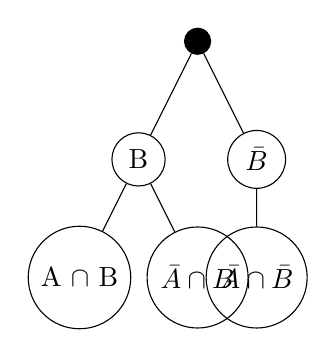
\begin{tikzpicture}[every node/.style={circle, draw=black}]
	[align=center, sibling distance=5cm]
	\node[fill=black]{}
		child { node{B} 
			child { node{A $\cap$ B} }
			child { node{$\bar{A} \cap B$} }
			}
		child{ node{$\bar{B}$} 
			%child{ node{$A \cap \bar{B}$} }
			child{ node{$\bar{A} \cap \bar{B}$} }
		       }
	;

\end{tikzpicture}

\end{document}